
%\newpage
%\section{논문에서 해결하고자 하는 구체적인 문제}\label{sec:bg}

%$$$$$$$$$$$$$$$$$$$$$$$$$$$$$$$$$$$$$$$$$$$$$$$$$$$$$$$$$$$$$$$$$$$$$$$$$$$$$$$$
% Paragraph : Linux Scalability : Fork intensive workload 문제점 설명 
%$$$$$$$$$$$$$$$$$$$$$$$$$$$$$$$$$$$$$$$$$$$$$$$$$$$$$$$$$$$$$$$$$$$$$$$$$$$$$$$$

%\begin{figure}[h]
%  \begin{subfigure}{0.45\textwidth}
%    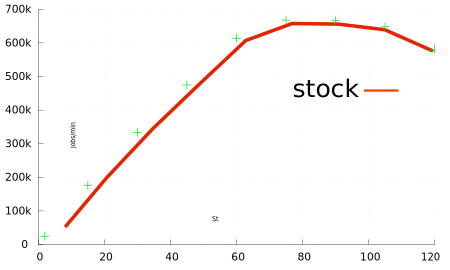
\includegraphics[width=\textwidth]{graph/aim7_default}
%    \caption{AIM7-multiuser scalability}
%  \end{subfigure}%
%  \begin{subfigure}{0.45\textwidth}
%    \includegraphics[width=\textwidth]{graph/lockstat}
%    \caption{Lock wait time on 120 core}
%  \end{subfigure}
%  \centering
%  \caption{Scalability of AIM7 multiuser and wait time to acquire locks on 120
  % core.
%  This workload simultaneously create many processes. The (a) shows up to 75
%  core, the stock Linux scales linearly, then it flattens out. The (b) left bar 
%  represents anonymous reader-writer semaphore causes a scalability bottleneck, 
%  and The (b) right bar shows file mapping reader-writer semaphore causes a
%  scalability bottleneck.}
%  \label{fig:aim7_default}
%\end{figure}


\begin{figure}[h]
    \centering
    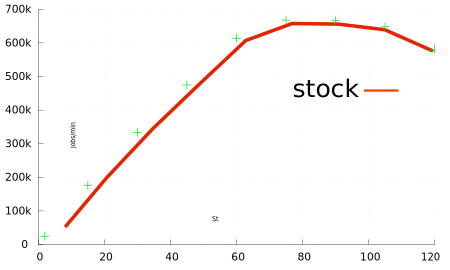
\includegraphics[width=0.8\textwidth]{graph/aim7_default}
    \caption{AIM7-multiuser 성능 확장성}
  \label{fig:aim7_default}
\end{figure}

\begin{figure}[h]
    \centering
    \includegraphics[width=0.8\textwidth]{graph/lockstat}
    \caption{120코어에서 락 때문에 기다리는 시간}
  \label{fig:aim7_default}
\end{figure}


%Applications' performance would be limited by the operating system kernel when 
%the operating system kernel does not scale
% well~\cite{Clements15SCR}~\cite{Boyd-WickizerCorey}.
%Linux has heavily optimized for multi-core operating systems.
%To analyze the current status of the operating system scalability,
%we measured the performance trends of the AIM7-multiuser benchmark on Linux
%with various CPU cores.
%The AIM benchmark has, until recently, been widely used in research area
%and the Linux community~\cite{Bueso2015STP}~\cite{Bueso2014MCS}.
%The AIM7-multiuser workload simultaneously creates many processes with
%disk-file operations, virtual memory operations, pipe I/O, and arithmetic
%operations.
%We used the temp filesystem to minimize the filesystem bottlenecks.
%The result of figure~\ref{fig:aim7_default}(a) shows that
%Linux shows significantly limited performance scalability when CPU core 
%exceeds 75.

운영체제 커널의 병렬화(parallelism)는 시스템 전체의 병렬화(parallelism)에서 가장 중요하다. 
만약에 커널이 확정성이 있지 않으면, 그 위에 동작하는 응용프로그램들도 역시 확장성이 있지
 않는다~\cite{Clements15SCR}~\cite{Boyd-WickizerCorey}.
우리는 이처럼 중요한 부분인 운영체제 커널 중 멀티코어에 최적화된 리눅스의 성능 확장성을 분석하기 위해, 
AIM7-multiuser를 가지고 성능 확장성을 실험해보았다.
AIM7은 최근에도 성능 확장성을 위해 연구(Research) 진영과 리눅스 커널 커뮤니티 진영에서도 활발히
 사용되고 있는 벤치마크 중 하나이다~\cite{Bueso2015STP}~\cite{Bueso2014MCS}.
AIM7-multiuser 워크로드는 동시에 많은 프로세스(Process)를 생성하며 수행되며, 디스크 파일(Disk File) 오퍼레이션,
 가상 메모리(Virtual Memory) 오퍼레이션, 파이프(Pipe), I/O(Input/Output) 그리고 수학 연산과 함께 수행한다.
우리는 파일 시스템의 성능 확장성(File system scalability)를 최소화하기 위해 
tempfs(Temp file system)를 사용하였다.
실험 결과 70코어까지 확장성을 가지나 그 이후에는 확장성이 떨어져 완만한 그래프를 보여준다. 


%$$$$$$$$$$$$$$$$$$$$$$$$$$$$$$$$$$$$$$$$$$$$$$$$$$$$$$$$$$$$$$$$$$$$$$$$$$$$$$$$
% Paragraph: Lockstat로 분석 결과 설명 
%$$$$$$$$$$$$$$$$$$$$$$$$$$$$$$$$$$$$$$$$$$$$$$$$$$$$$$$$$$$$$$$$$$$$$$$$$$$$$$$$

%To understand the sources of scalability bottleneck on 120 core systems, we
% profiled a lock contention using the \code{lock\_stat}~\cite{LOCKSTAT}, a Linux kernel lock profiler that reports how
%long each lock is held and the wait time to acquire the lock.
우리는 성능 확장성에 근본적인 문제를 분석하기 위해, 문제가 있는 120코어에서 리눅스의
 \code{lock\_stat}~\cite{LOCKSTAT}를 이용하여 락 경합을 분석하였다.
 \code{lock\_stat}는 리눅스 커널에 있는 락 프로파일러(profiler)이며, 얼마나 스레드(Thread)가 락을 보유하고 
 락을 얻기 위해 쓰레드가 얼마나 기다리고 있지를 보여준다.
%The figure~\ref{fig:aim7_default}(b) shows the cost of acquiring the lock for
% the AIM7-multiuser running on a 120 core system.
먼저 멀티 프로세스 기반의 벤치마크인 AIM7을 동작시키고 동시에 120코어 대해서 락 경합을 분석하면 
그림 ~\ref{fig:aim7_default}과 같은 결과를 가진다. 
%Results of the \code{lock\_stat} that the main source of lock contention was
% the anonymous reverse mapping semaphore(\code{anon\_vma->rwsem}), 
%which was caused by simultaneously creating a number of processes.
AIM7 벤치마크의 경우 상당히 많은 부분이 익명 VMA에서 쓰기 락 경합이 발생한다. 
이는 리눅스 역 매핑(reverse mapping)을 효율적으로 수행하기 위한 자료구인 익명 역 매핑 세마포어(semaphore)
(\code{anon\_vma->rwsem}) 수많은 fork에 의해 프로세스를 생성하면서 발생하는 락 경합 문제이다.
이러한 역 페이지 매핑(revsers page mapping)은 리눅스가 fork(), exit(), and mmap() 시스템
콜(system call)을 사용할 때 페이지(page) 정보를 업데이트한다.


 \begin{figure}[h]
    \centering
    \includegraphics[width=0.8\textwidth]{fig/anon_vma_rmap}
    \caption{anonymous 역 매핑의 문제}
  \label{fig:anon_vma_rmap}
\end{figure}


%The reverse page mapping records page information when using fork(), exit() and
%mmap() system call to find all page table entries.
%To understand further bottlenecks, we intentionally removed the kernel codes
% causing anonymous reverse mapping which has been revealed as the most significant source of the problem.
%conducted a workaround by removing
%anonymous reverse mapping relative code in the part of the Linux fork with page-swap off
%because of avoiding the Linux page reclaiming.
%When the anonymous reverse mapping code was removed, 
%the second major source of the bottleneck was file 
%reverse mapping reader-writer semaphore(\code{mapping->i\_mmap\_rwsem}).
다음으로 우리는 익명 역 매핑의 락 경합을 줄이기 위해, 임시로 fork에서 익명 역 매핑를 호출하는 부분과 
읽기와 관련 있는 페이지 스왑(page swap)이 안되도록 하고, 120코어를 대상으로 다시 락 경합을 분석하여 보았다.
이때 부터 그동안 상대적으로 가려졌던 파일 역 매핑에서 많은 락 경합이 발생되었다.
본 연구의 분석 결과 둘 중 하나가 아니라 두 가지 락 모두 fork의 성능 확장성 문제를 일으킨다.

 \begin{figure}[h]
    \centering
    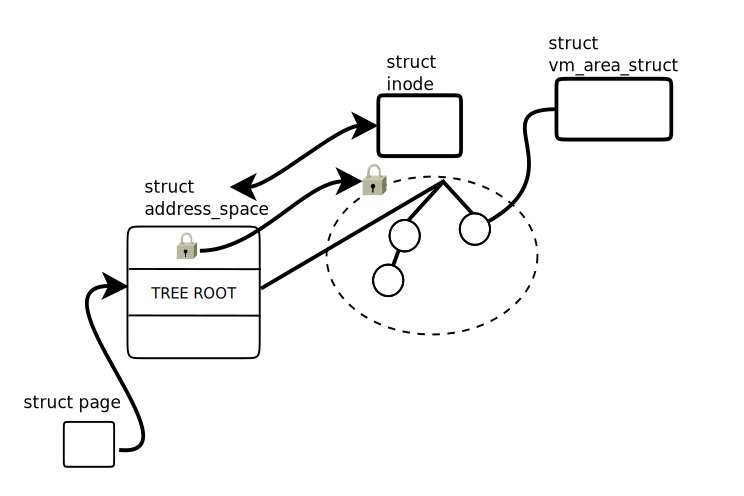
\includegraphics[width=0.8\textwidth]{fig/file_rmap_default}
    \caption{파일 역 매핑의 문제}
  \label{fig:file_rmap_default}
\end{figure}



%$$$$$$$$$$$$$$$$$$$$$$$$$$$$$$$$$$$$$$$$$$$$$$$$$$$$$$$$$$$$$$$$$$$$$$$$$$$$$$$$
% Paragraph : 리눅스 reverse page map의 write serialization 문제점
%$$$$$$$$$$$$$$$$$$$$$$$$$$$$$$$$$$$$$$$$$$$$$$$$$$$$$$$$$$$$$$$$$$$$$$$$$$$$$$$$

%Our background study showed that both the anonymous reverse mapping
%reported from the Linux community~\cite{Andi2011adding} and the file reverse
% mapping reported from S.
%Boyd-Wickizer~\cite{SilasBoydWickizerPth} are significant factors in fork
% scalability problem.
%Thus, in order to perfect scalability of the fork, both the
%file reverse mapping and the anonymous reverse mapping should be executed
%concurrently without any lock.
%In fact, the fundamental scalability problem of reverse mapping is their
%serialized update operations because operating systems are serialized at
%the update operations.
이러한 익명 역 페이지 매핑은 리눅스 커뮤니티에서 잘 알려진 락 경합
문제~\cite{Andi2011adding}이고, 파일 페이지 역 매핑에 대한 락
경합 문제는 S.Boyd-Wickizer~\cite{SilasBoydWickizerPth} OpLog 논문을 통해
 fork의 확장성 문제의 중요한 원인으로 제시한 부분이다.
즉 두 가지 모두 개선해야지 fork의 성능 확장성이 향상 된다. 

\begin{figure}[h]
    \centering
    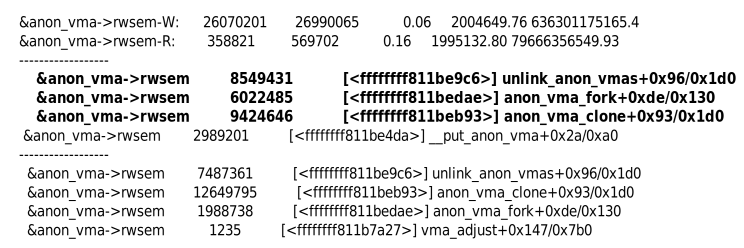
\includegraphics[width=0.8\textwidth]{fig/anon_vma_func}
    \caption{120코어에서의 lock\_stat 결과 분석}
  \label{fig:anon_vma_func}
\end{figure}



 \begin{figure}[h]
    \centering
    \includegraphics[width=0.8\textwidth]{fig/update}
    \caption{업데이트 직렬화의 문제}
  \label{fig:update}
\end{figure}



%$$$$$$$$$$$$$$$$$$$$$$$$$$$$$$$$$$$$$$$$$$$$$$$$$$$$$$$$$$$$$$$$$$$$$$$$$$$$$$$$
% Paragraph : update heavy한 상황에 대한 설명과 해결 방법에 대한 설명
%$$$$$$$$$$$$$$$$$$$$$$$$$$$$$$$$$$$$$$$$$$$$$$$$$$$$$$$$$$$$$$$$$$$$$$$$$$$$$$$$

%Existing research accomplishments to achieve scalable concurrent update in many
%core systems are categorized into two methods:
%non-blocking
%algorithms~\cite{Harris2001Lockfree}~\cite{Fomitchev2004Lockfree}~\cite{Timnat2012}
% in early stages and log-based algorithms.
%In non-blocking algorithms, update operation observes against the current
%value in global data structure, and they execute an atomic compare and
% swap(CAS) to compare the against value.
%When the value has been overridden, the updater must be retried.
%Consequently, both the repeated global CAS operation and the iteration loop
% caused by CAS fails will result in bottlenecks due to inter-core communication
%overheads~\cite{SilasBoydWickizerPth}.
%To overcome the problem of cache coherence systems, log-based methods are
%proposed.
%Our research also uses a log-based deferred design that alows concurrent
%updates to scale, so that multiprocessed applications can scale to large
% numbers of cores.
이러한 높은 업데이트 비율 때문에 발생하는 업데이트 직렬화 문제에 대한 해결 방법들은
그동안 여러 방법이 제안되었다. 
해결 방법들은 동시적 업데이트를 위한, 논블락킹 자료구조(non-blocking data structure)를 이용하는 
방식과 로그 기반(log-based) 알고리즘을 사용하는 방법이 있다.
논블락킹 알고리즘들은 하드웨어 동기화 원자적(hardware synchronized atomic) 연산들을 활용하여
동시적으로 업데이트와 읽기 명령어를 수행하게한 자료구조이다.
예를들어, 논블락킹 알고리즘들은 업데이트 명령어 수행전에 전역 변수를 지켜본 후, 업데이트를 
원자적인 CAS(Compare And Swap) 명령으로 전역 변수가 변경되었는지 확인과 저장하는 읽을 원자적으로 
수행한다. 
이때 해당 전역변수가 수정되었다면, 업데이트 명령어는 다시 처음부터 수행하여 다른 스레드가 변경을 
안 할때까지 같은 일을 수행하는 방법이다.  
하지만 이러한 방법도 결국 전역 공유 메모리 주소에 다수의 CAS로 접근하여
병목현상이 생긴다. 이것은 결국 캐시 커뮤니케이션 오버헤드를 만든다~\cite{SilasBoydWickizerPth}.
최근에는 전역 공유 메모리 주소에 다수의 CAS(Compare And Swap)로 접근하여
발생하는 병목현상을 줄인 로그 기반 방법들이 연구되고 있다.
우리의 LDU도 이러한 로그 기반 방법을 활용하였다.

%$$$$$$$$$$$$$$$$$$$$$$$$$$$$$$$$$$$$$$$$$$$$$$$$$$$$$$$$$$$$$$$$$$$$$$$$$$$$$$$$
%Paragraph : Log 기반의 알고리즘 대략적인 설명 
%$$$$$$$$$$$$$$$$$$$$$$$$$$$$$$$$$$$$$$$$$$$$$$$$$$$$$$$$$$$$$$$$$$$$$$$$$$$$$$$$

%Log-based algorithm is that when update operations occur, it logs the update
%operation and applies the all operation logs to the data structure
%before read operation, so reader can read up to date data structure.

%The log-based algorithms are
%a suitable solution for the update-heavy data structure because they allow
%update operations to proceed with a coarse-grained update lock or without
%update locks.
%The benefit of avoiding a fine-grained update lock can eliminate the overhead
% of acquiring a lock that requires fetching the lock's cache line.
%Thus, it reduces the cache communication traffic;a contended cache line on
%many-core processors can take hundreds of cycles to fetch from a remote
%core~\cite{AustinTClements2012RCUBalancedTrees}, and these techniques can be
% easily applied to other data structures.
%In addition to avoiding fine-grained lock and easily applying the
%other data structures, a log-based method can remove an existing
%operation log rather than actually executing a operation log.

로그 기반 알고리즘은 업데이트 비율이 많은 자료구조에 적합한 알고리즘이다. 
로그 기반 알고리즘은 락을 피하기 위해 업데이트가 발생하면, 자료구조의 업데이트 
명령어(삽입 또는 삭제)를 함수 인자(argument)와 함께 저장하고, 주기적 또는 읽기 명령이
 수행하기 전에 그동안 저장된 로그를 수행하는 방법이다.
이러한 로그 기반 방법은 마치 CoW(Copy on Write)와 유사하다.
즉, 읽기 전에 저장된 쌓여있는 로그가 수행됨으로 읽기가 간혈적으로 수행되는 자료구조에 적합한 방법이다.



\begin{figure}[h]
    \centering
    \includegraphics[width=0.8\textwidth]{fig/oplog_log}
    \caption{로그 기반 방법 중 로그의 내용}
  \label{fig:oplog_log}
\end{figure}



업데이트 비율이 많은 자료구조를 위한 로그 기반 방법은 총 4가지의 장점을 가진다. 
첫째로, 업데이트가 수행하는 시점 즉 로그를 저장하는 순간에는 락이 필요가 없다. 
따라서 업데이트를 동시적으로 수행할 수 있을 뿐만 아니라, 락 자체가 가지고 있는 캐시 메모리 오버헤드를 
줄일 수 있다. 
둘째로, 저장된 순차적인 업데이트 명령을 하나의 코어에서 수행하기 때문에, 캐시 지역성이 높아진다.
셋째로, 큰 수정 없이 기존 여러 데이터(tree, queue) 자료구조에 쉽게 적용할 수 있는 장점이 있다.
마지막으로 저장된 로그를 실제 수행하지 않고, 여러 가지 최적화 방법을 사용하여 적은 
명령으로 로그를 줄일 수 있다. 
LDU도 로그 기반 방법을 따른다. 그러므로 앞에서 설명한 로그 기반 방법의 장점을 모두 가짐과 동시에
업데이트 순간 삭제 가능한 로그를 지움으로 성능이 향상된다.

%One notable recent research accomplishment regarding log-based approach is
%the OpLog proposed by S. Boyd-Wickizer \textit{et al.}.
%The OpLog utilizes representative distributed systems management concepts(e.g.,
% Google spanner's synchronized clocks scheme~\cite{Corbett2013SGG}) and proposes the log-based algorithm to shared-memory systems.
%The OpLog shows significant improvement in performance scalability for
% update-heavy operating system data structures.
%Though the OpLog forms an important basis for another step of improvement in
% performance scalability problem in many core systems, it still has limitation that it's 
%synchronized time-stamp counters might cause additional overhead during log
% management process.
%The OpLog using the synchronized time-stamp counters method may incur
%time-stamp merging and ordering process.
%Consequently, when core counts increases, the time-stamp merging and ordering
%process may require sequential processing, which can limit scalability and
%performance.
%For example, if cores counts are 1000 and per-core logs counts are 10, 
%because each log searches all core's log, 

\begin{figure}[h]
    \centering
    \includegraphics[width=0.8\textwidth]{fig/oplog_max}
    \caption{동기화된 타임스탬프 카운터 머징에 따른 오버헤드}
  \label{fig:oplog_log}
\end{figure}


동기화된 타임스탬프 카운터 기반의 퍼코어 로그를 활용한 동시적 업데이트방법은 결국
 타임스탬프 병합 작업을 일으킨다.
특히 코어 수가 늘어 날 경우, 퍼코어 로그를 자료 구조에 적용하는 과정에서 추가적인 
순차적인 프로세싱이 요구된다.
이것은 확장성과 성능을 저해한다. 




